\section{Comparison with State-of-the-Art Methods}
To evaluate the performance of our models in the context of state-of-the-art solutions, we compared our results to several notable studies. These works employ a diverse range of techniques, from traditional machine learning to advanced deep learning models, allowing us to position our findings within the current research landscape.

\subsection{Short-Term Residential Load Forecasting based
on LSTM Recurrent Neural Network}
In the study "Short-Term Residential Load Forecasting based
on LSTM Recurrent Neural Network"\cite{kong2019short} the authors apply LSTMs to forecast the short-term electricity consumption of individual residential households. 

The authors apply multiple LSTM layers staked on top of each other. These layers are responsible for learning the temporal dependencies between past energy consumption and future predictions. The use of multiple LSTM layers provides the learning of more complex relationships as the depth increases. After the LSTM layers have learned, the output passes through a final feedforward neural network that predicts the energy consumption for the target time step as can be seen in the following image.

\begin{figure}[!h]
    \centering
    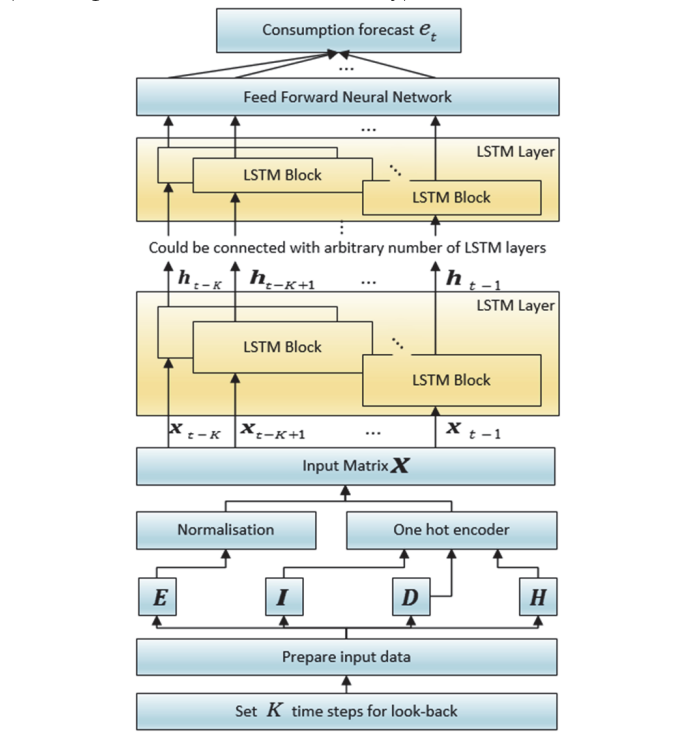
\includegraphics[width=0.75\linewidth]{images/study_lstm.png}
    \caption{Short-term residential load forecasting model architecture\cite{kong2019short}}
    \label{fig:architecture_lstm_study}
\end{figure}

Comparing this architecture with our study's, our architecture is much more simple yet effective for the problem we have at hand. It contains a single LSTM layer, and then a dense layer. Our model has achieved great results and increasing its complexity does not mean we would get better ones. An evidence to this conclusion can be understood from the behaviour of the loss function or \(R^2\) over epochs. We can see the model practically stopped learning in only four epochs which indicates the model is learning very well.

The "Short-Term Residential Load Forecasting(...)" study used the Mean Absolute Percentage Error (MAPE) metric for evaluating the accuracy of the predictions, in contrast to our study which preferred the MAE, MSE, RMSE, and \(R^2\). In conclusion, this comparison highlights that not always a complex model architecture is needed to achieve great results.


\subsection{Comparative Analysis of our results with Existing Studies}

To contextualize the performance of our models, we compare them against notable existing works in the literature. The comparison focuses on key evaluation metrics such as Mean Absolute Error (MAE), Mean Squared Error (MSE), Root Mean Squared Error (RMSE), and the coefficient of determination (R²).

\begin{table}[H]
\centering
\caption{Performance Metrics from Ahmad et al. (2017)~\cite{ahmad2017random}}
\begin{tabular}{llcccc}

 \textbf{Model} & \textbf{RMSE (Val)} & \textbf{R² (Val)} & \textbf{RMSE (Test)} & \textbf{R² (Test)} \\
RF & 0.048 & 0.9968 & 0.0559 & 0.9966 \\
ANN & 0.043 & 0.9975 & 0.0493 & 0.9973 \\
\end{tabular}
\label{tab:ahmad2017_results}
\end{table}

\begin{table}[H]
\centering
\caption{Performance Metrics from Dinh et al. (2023)~\cite{khan2024image}}
\begin{tabular}{llcccc}

\textbf{Dataset} & \textbf{Model} & \textbf{MAE\textsubscript{t}} & \textbf{RMSE\textsubscript{t}} & \textbf{MAE} & \textbf{RMSE} \\

{ DF1} 
& M-LSTM &  0.75  &  1.15  & 1.08 & 1.37 \\
& LSTM   & 1.30 & 1.47 & 1.35 & 1.58 \\
& Bi-LSTM & 1.46 & 1.85 & 1.53 & 1.63 \\
& Linear Reg. & 1.40 & 1.53 & 1.40 & 1.50 \\
{ DF2}  
& M-LSTM &  0.49  &  0.74  & 0.84 & 0.96 \\
& LSTM   & 1.47 & 1.66 & 1.89 & 2.00 \\
& Bi-LSTM & 1.45 & 1.16 & 1.89 & 2.06 \\
& Linear Reg. & 0.60 & 0.75 & 1.21 & 1.52 \\
{ DF3}  
& M-LSTM &  0.66  &  0.85  & 0.69 & 0.87 \\
& LSTM   & 0.79 & 0.95 & 0.67 & 0.94 \\
& Bi-LSTM & 1.61 & 2.15 & 1.23 & 1.92 \\
& Linear Reg. & 0.84 & 1.18 & 0.73 & 0.90 \\

\end{tabular}
\label{tab:dinh2023_results}
\end{table}



\begin{table}[H]
\centering
\caption{Comparison of Test Set Performance Metrics Across our Models}
\begin{tabular}{lcccc}

\textbf{Model} & \textbf{MAE} & \textbf{MSE} & \textbf{RMSE} & \textbf{R²} \\
 Random Forest (Tuned)  & 0.0744 & 0.0237 & 0.1541 & 0.9910 \\
 FNN 1  & 0.1445 & 0.0467 & 0.2161 & 0.9823 \\
 FNN 2  & 0.1312 & 0.0452 & 0.2125 & 0.9829 \\
 FNN with Grouped Features  & 0.1251 & 0.0430 & 0.2073 & 0.9837 \\
 LSTM (Best)  &  0.0930  &  0.0320  &  0.1800  &  0.9880  \\
\end{tabular}
\label{tab:comparison_test_metrics}
\end{table}

Table~\ref{tab:ahmad2017_results} presents the results reported by Ahmad et al. (2017)~\cite{ahmad2017random}, who utilized Random Forest and Artificial Neural Networks (ANN) to predict energy consumption. Their ANN model demonstrated outstanding performance, achieving an RMSE of 0.0493 and an R² of 0.9973 on the test set—surpassing all our models in these two metrics. It is important to note, however, that their experimental setup differs considerably from ours, particularly in terms of input feature types, data resolution, and preprocessing steps. These differences limit the extent to which direct performance comparisons can be made.

In a more recent study, Dinh et al. (2023)~\cite{khan2024image} explored several recurrent neural network variants, including standard LSTM, bidirectional LSTM (Bi-LSTM), and multivariate LSTM (M-LSTM), for time-series forecasting of commercial building energy usage. As shown in Table~\ref{tab:dinh2023_results}, their best-performing models yielded MAEs ranging from 0.49 to 1.53 and RMSEs from 0.74 to 2.06, depending on the dataset. When compared to our best LSTM model (MAE = 0.0930, RMSE = 0.1800), our results demonstrate notably superior accuracy. This improvement may be attributed to targeted preprocessing and feature grouping. Still, such comparisons must be contextualized within the differences in datasets, time horizons, and modeling goals.

Finally, Table~\ref{tab:comparison_test_metrics} summarizes the performance of all our proposed models on the test set. Among them, the tuned Random Forest model achieved the highest R² (0.9910), indicating strong explanatory power. Meanwhile, the LSTM model offered the most balanced performance, combining a low MAE and RMSE with robust generalization. When considered alongside prior studies, our models not only show competitive results but also reinforce the effectiveness of combining classic ensemble methods with modern deep learning techniques in energy consumption prediction tasks.

\section{Future Work}

While the current study demonstrates promising results in predicting energy consumption using various machine learning and deep learning models, several avenues remain for future exploration and improvement.

First, although we focused primarily on unidirectional LSTM architectures, future work could investigate the use of \textbf{Bidirectional LSTM (Bi-LSTM)} and \textbf{Multivariate LSTM (M-LSTM)} models. These architectures have shown potential in related literature for capturing complex temporal dependencies by incorporating both forward and backward sequences, as well as leveraging multiple input features more effectively. Given our positive results with grouped features, a multivariate time-series approach could further improve model accuracy and robustness.

Additionally, our current models were trained on a unified dataset that includes buildings with a variety of \textbf{primary use types}. This generalization can limit performance, especially if usage patterns vary significantly between categories (e.g., schools vs. hospitals vs. offices). A logical extension of our work would involve \textbf{training specialized models per primary use category}, allowing each model to learn domain-specific patterns and seasonal trends. This segmentation could lead to more precise and tailored energy forecasts.

In summary, the foundation laid by this study can be expanded upon through architectural innovations, data stratification, and richer contextual inputs, paving the way for even more accurate and adaptive energy forecasting models.
